\subsection{Abstraction} \label{section:license-abstraction}
All license verification libraries are working inside the application and query a trusted source.
They do not prevent redistribution or copying but enforce the authorization when the application is run.
The result of the verification is always binary, either access is granted or it is prohibited.
In the further analysis it will be shown that this binary mechanism is an easy target for attacks, such as executed by \gls{luckypatcherg}.
\newline
The functionality of the libraries can be abstracted as a simple \textit{yes/no} check as seen in figure~\ref{fig:verificationNow}.
\begin{figure}[h]
    \centering
    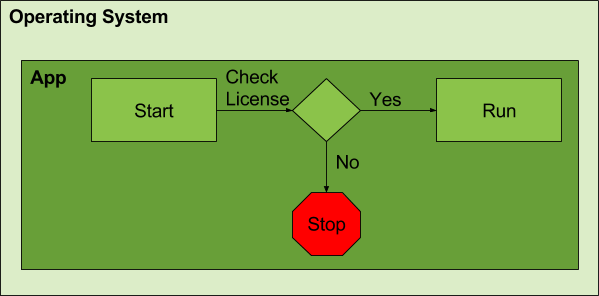
\includegraphics[width=0.8\textwidth]{data/verificationNow.png}
    \caption{Abstraction of the current license verification mechanism. The library is represented by (1)}
    \label{fig:verificationNow}
\end{figure}
